%%%%%%%%%%%%%%%%%%%%%%%%%%%%%%%%%%%%%%%%%
% University/School Laboratory Report
% LaTeX Template
% Version 3.1 (25/3/14)
%
% This template has been downloaded from:
% http://www.LaTeXTemplates.com
%
% Original author:
% Linux and Unix Users Group at Virginia Tech Wiki 
% (https://vtluug.org/wiki/Example_LaTeX_chem_lab_report)
%
% License:
% CC BY-NC-SA 3.0 (http://creativecommons.org/licenses/by-nc-sa/3.0/)
%
%%%%%%%%%%%%%%%%%%%%%%%%%%%%%%%%%%%%%%%%%

%----------------------------------------------------------------------------------------
%	PACKAGES AND DOCUMENT CONFIGURATIONS
%----------------------------------------------------------------------------------------

\documentclass{article}


\usepackage{siunitx} % Provides the \SI{}{} and \si{} command for typesetting SI units
\usepackage{graphicx} % Required for the inclusion of images
\usepackage{amsmath} % Required for some math elements 
\usepackage{url}
\usepackage{algorithm}
\usepackage{algpseudocode}
\usepackage{amsmath}
\usepackage{graphics}
\usepackage{epsfig}
\usepackage{indentfirst}
\usepackage{textcomp}
%\usepackage[showframe=true]{geometry}
\usepackage{geometry}
\usepackage{changepage}
\usepackage[flushleft]{threeparttable}
\usepackage{graphicx}



\newcommand{\tabincell}[2]{\begin{tabular}{@{}#1@{}}#2\end{tabular}}  
\renewcommand{\labelenumi}{\alph{enumi}.} % Make numbering in the enumerate environment by letter rather than number (e.g. section 6)

\newcounter{algsubstate}
\renewcommand{\thealgsubstate}{\alph{algsubstate}}
\newenvironment{algsubstates}
{\setcounter{algsubstate}{0}%
	\renewcommand{\State}{%
		\stepcounter{algsubstate}%
		\Statex {\footnotesize\thealgsubstate:}\space}}
{}




\newenvironment{itquote}
{\begin{quote}\itshape}
	{\end{quote}\ignorespacesafterend}
\newenvironment{itpars}
{\par\itshape}
{\par}



%\usepackage{times} % Uncomment to use the Times New Roman font

%----------------------------------------------------------------------------------------
%	DOCUMENT INFORMATION
%----------------------------------------------------------------------------------------

\title{ Reconstructing collapsed complex network to find most influential nodes  } % Title

\author{Fengkuangtian \textsc{Zhu}} % Author name

\begin{document}
	
	\maketitle % Insert the title, author and date
	
	
	
	\begin{center}
		\begin{tabular}{c}
			Solution of Datacastle Master Competition	\\
			Team ID: zhfkt 
		\end{tabular}
	\end{center}
	
	% If you wish to include an abstract, uncomment the lines below
	\begin{abstract}
		This solution paper is to demonstrate the solution of algorithm in identifying vital nodes in complex networks for Datacastle Master Competition . Compared with traditional algorithms including Betweenness\cite{wikiBetweennesscentrality}, Closeness\cite{wikiClosenesscentrality}, PageRank\cite{wikiPageRank}, Degree\cite{wikiCentrality} and Collective Influence\cite{morone2015influence}\cite{morone2016collective}, the new proposed algorithm of reconstructing collapsed complex network to find most influential nodes is able to achieve the better performance on the 8 competition datasets in terms of robustness\cite{schneider2011mitigation} and speed. The new implementation by c++ of the popular algorithm Collective Influence (CI) is introduced as well, named ComplexCi. All code in the paper can be found at the link https://github.com/zhfkt/ComplexCi \cite{zhfktgithub} \cite{zhfkt2017887989}
	\end{abstract}

	\section{Introduction}


	Overall, the target of finding most influential nodes algorithm is to give a ranking list of nodes according to their importance. The top-ranked nodes will have more importance. We can remove the nodes from the top-ranked ones in the ranking list generated by algorithm and calculate the size of giant component after each removal, which will break down the network into many disconnected pieces. The ratio of giant component will reach zero with the one-by-one removal operation finally. Therefore, the better algorithm, the sooner the network will collapse to the zero giant component with smaller count of provided nodes. Robustness \cite{schneider2011mitigation} is introduced in the Competition to quantify the performance of ranking nodes methods. 
	
	There are several traditional algorithms such as Betweenness\cite{wikiBetweennesscentrality}, Closeness\cite{wikiClosenesscentrality}, PageRank\cite{wikiPageRank}, Degree\cite{wikiCentrality} and Collective Influence\cite{morone2015influence}\cite{morone2016collective} for the target. In this paper, the new algorithm is proposed for reconstructing collapsed complex network in order to find most influential nodes. Compared with the traditional algorithms, the new method is able to achieve the better performance in terms of robustness and speed. 
	
	This solution paper is organized as follows. In Section 2, DataCastle Master Competition background describes the target of this solution paper. In Section 3, several traditional algorithms are used to investigate the performance of 8 competition datasets as comparative algorithms. In Section 4, the suggested Collective Influence with optimal percolation is applied to get the advanced performance. The new implementation by C++ of CI , named ComplexCi , is also introduced. In Section 5, new proposed reconstructing algorithm is developed , and then verified on 8 datesets in performance in the experiments section. Lastly, the conclusions of new algorithms and this competition are provided with outlook. All the code in this paper can be found at the link https://github.com/zhfkt/ComplexCi \cite{zhfktgithub} \cite{zhfkt2017887989}



	\section{DataCastle Master Competition background}
	
	From \cite{masterCompetitionbackground} , the detaild of Master Competition background held by DataCastle are described below:
	
	\begin{itquote}
		
		Disparate networks, including social networks, communication networks and biological networks, are playing an increasingly important role on natural and social-economic systems. A core problem, therein, is to measure the significance of individual nodes. For instance, a super spreader in HongKong triggered transmission of SARS to a significantly greater number of other people than 100 normal infected persons; a rumour re-tweeted by a celebrity may spread much broader than that by an obscure person.
		
		Therefore it is necessary to develop a method to identify the virulence genes in large-scale gene regulatory networks, to find the super-spreaders in large-scale social networks, and to detect the key enterprises with serious systematic financial risk in large-scale financial networks.
		
		Those tasks could be formalized as a generic challenge that is identifying vital nodes in networks that are important for sustaining connectivity. This challenge, aka optimal percolation, is a well-documented issue in network science. With great anticipation of making big progress on this problem, we successfully invited some experts and hope the great participants will create novel and effective solutions.  		
	\end{itquote}

	
	The competition provides 4 real networks from different fields, including autonomous system network, Internet network, road network and social network, and 4 classical artificial networks as well (total 8 datasets). The numbers of nodes of these networks range from 0.7 million to 2 million. All of them are considered as undirected networks. Table \ref{tab:table1} shows the network name and corresponding numbers of nodes.
	

	\begin{table}[!htbp]
	
	\centering
	\caption{ Network name and corresponding numbers of nodes}
	\label{tab:table1}
	%\begin{adjustwidth}{0.0cm}{}
		\begin{tabular}{|c|c|c|c|c|c|c|c|c|}
			\hline
			\textbf{Network} & \textbf{model1} & \textbf{model2} & \textbf{model3} & \textbf{model4} & \textbf{real1} & \textbf{real2} & \textbf{real3} & \textbf{real4} \\ \hline
			\textbf{Number} & 1039722         & 1083568         & 997663          & 1001733         & 1694616        & 1957027        & 426485         & 855802         \\ \hline
		\end{tabular}
	%\end{adjustwidth}
	\end{table}

	For the experiments in this paper, datasets are all verified on the default 4-core CPU machine (Intel Xeon E5-2667v4 Broadwell 3.2 GHz) in 8G memory if I don't mention especially.


	\section{Experiments on the traditional algorithms}
	
	In this section, tradition algorithms of Betweenness\cite{wikiBetweennesscentrality}, Closeness\cite{wikiClosenesscentrality}, Degree\cite{wikiCentrality} and PageRank\cite{wikiPageRank}  will be verified on 8 Datacastle datasets. 

	\subsection{Betweenness}
	
	Betweenness is a centrality measure of a vertex within a graph . Betweenness centrality quantifies the number of times a node acts as a bridge along the shortest path between two other nodes \cite{wikiBetweennesscentrality}\cite{freeman1977set}. Here betweenness is used to find the most influential nodes in the complex networks. Robustness value after applying Betweenness on 8 competition datasets is shown in the Table \ref{tab:table2}
	
	
	\begin{table}[!htbp]
	\small\begin{adjustwidth}{-1.3cm}{}		
		\begin{threeparttable}
			\centering
			\caption{Robustness value and time after applying Betweenness on 8 competition datasets}
			\label{tab:table2}
		
			\begin{tabular}{|c|c|c|c|c|c|c|c|c|c|}
				\hline
				\textbf{Betweenness}          & \textbf{model1} & \textbf{model2} & \textbf{model3} & \textbf{model4} & \textbf{real1} & \textbf{real2} & \textbf{real3} & \textbf{real4} & \textbf{Total} \\ \hline
				\textbf{Robustness Score} & 0.3125          & 0.2678          & 0.4484          & 0.1952          & 0.1101         & 0.0064         & 0.1582         & 0.1076         & 1.6060         \\ \hline
				\textbf{Time}     & 201733s          & 187508s          & 270524s          & 231936s         & 624256s         & 327145s         & 109726s         & 109685s         & 2062513s        \\ \hline
			\end{tabular}
				\begin{tablenotes}
					\small
					\item\textit{8 datasets are all verified in parallel supported by GraphTools \cite{peixotographtool2014}}
				\end{tablenotes}			
	 	\end{threeparttable}
	\end{adjustwidth}
\end{table}
	
	
	Although Betweenness is supported to be executed in utilizing all CPU cores in parallel by GraphTools \cite{peixotographtool2014} to boost , it is still obvious that Betweenness spends nearly 24 days $\simeq$ 1 month in completing the verification of 8 datasets. Considered the time and effort , robustness value of Betweenness is not very well. Betweenness fails to process the networks of million scale to find most influential nodes.
	
	\subsection{Closeness}	
	
	
	In a connected graph, the Closeness centrality of a node is the average length of the shortest path between the node and all other nodes in the graph. Thus the more central a node is, the closer it is to all other nodes \cite{wikiClosenesscentrality}\cite{bavelas1950communication} . Here closeness is also used to find the most influential nodes in the complex networks. Robustness value after applying Closeness on 8 competition datasets is shown in the Table \ref{tab:table3}
	
	\begin{table}[!htbp]
		\begin{adjustwidth}{-1.3cm}{}		
			\begin{threeparttable}
				\centering
				\caption{Robustness value and time after applying Closeness on 8 competition datasets}
				\label{tab:table3}
				
				\begin{tabular}{|c|c|c|c|c|c|c|c|c|c|}
					\hline
					\textbf{Closeness}          & \textbf{model1} & \textbf{model2} & \textbf{model3} & \textbf{model4} & \textbf{real1} & \textbf{real2} & \textbf{real3} & \textbf{real4} & \textbf{Total} \\ \hline
					\textbf{Robustness Score} & 0.4140          & 0.3765          & 0.4624          & 0.3717          & 0.2495         & 0.4454         & 0.2738         & 0.2868         & 2.8801         \\ \hline
					\textbf{Time}     & 63095s           & 63552s           & 71382s           & 46107s           & 136945s         & 161397s         & 17992s          & 31564s          & 592034s         \\ \hline								
				\end{tabular}
				\begin{tablenotes}
					\small
					\item\textit{8 datasets are all verified in parallel supported by GraphTools \cite{peixotographtool2014} on the 8-core CPU machine (Intel Xeon E5-2667v4 Broadwell 3.2 GHz) in 16G memory. Please notice that CPU cores in verifying Closeness are 8 cores, double than the default CPU cores of machine mentioned above}
				\end{tablenotes}			
			\end{threeparttable}
		\end{adjustwidth}
	\end{table}
	
	Similar with Betweenness , although Closeness algorithm is supported to be executed in utilizing all CPU cores in parallel by GraphTools to boost , it is still obvious that Closeness spends nearly 7 days $\simeq$ 1 week in completing the verification of 8 datasets. Considered the time and effort , robustness value of Closeness is also not very well. Closeness fails to process the networks of million scale to find most influential nodes as Betweenness .
	
	
	\subsection{PageRank}	
	
	
	PageRank works by counting the number and quality of links to a page to determine a rough estimate of how important the website is. The underlying assumption is that more important websites are likely to receive more links from other websites \cite{wikiPageRank}\cite{page1999pagerank}. Here PageRank is also used to find the most influential nodes in the complex networks. Robustness value after applying PageRank on 8 competition datasets is shown in the table \ref{tab:table4}
	
	\begin{table}[!htbp]
	\begin{adjustwidth}{-1.3cm}{}		
		\begin{threeparttable}
			\centering
			\caption{Robustness value and time after applying PageRank on 8 competition datasets}
			\label{tab:table4}
			
			\begin{tabular}{|c|c|c|c|c|c|c|c|c|c|}
				\hline
				\textbf{PageRank}          & \textbf{model1} & \textbf{model2} & \textbf{model3} & \textbf{model4} & \textbf{real1} & \textbf{real2} & \textbf{real3} & \textbf{real4} & \textbf{Total} \\ \hline
				\textbf{Robustness Score} & 0.2435          & 0.2043          & 0.4267          & 0.1469          & 0.0522         & 0.1364         & 0.1430         & 0.0832         & 1.436          \\ \hline
				\textbf{Time}     & 701s             & 686s             & 750s             & 552s             & 2106s           & 1845s           & 918s            & 663s            & 8221s           \\ \hline							
			\end{tabular}
			\begin{tablenotes}
				\small
				\item\textit{8 datasets are all verified in single thread supported by GraphTools \cite{peixotographtool2014} }
			\end{tablenotes}			
		\end{threeparttable}
	\end{adjustwidth}
	\end{table}

		
	Compared with Betweenness and Closeness , algorithm PageRank gets much better result in robustness and speed. Especially , PageRank just runs in single thread and uses less resources than betweenness and closeness. Robustness value of PageRank is 1.436 and also better than Betweenness and Closeness 
	
	\subsection{Degree}		

	Historically first and conceptually simplest is degree centrality, which is defined as the number of links incident upon a node . i.e. the number of ties that a node has \cite{wikiCentrality}. The nodes are ranked by degree, and sequentially removed starting from the node of highest degree. The concept of High Degree Adaptive (HDA) is proposed in the \cite{morone2015influence} as a better strategy which is a slightly different from the original Degree algorithm. Degree of the remaining nodes in the adaptive version will be recomputed after each node removal. HDA is used here to find the most influential nodes in the complex networks. Robustness value after applying HDA on 8 competition datasets is shown in the table \ref{tab:table5}
	

		
	\begin{table}[!htbp]
		\begin{adjustwidth}{-1.3cm}{}		
			\begin{threeparttable}
				\centering
				\caption{Robustness value and time after applying HDA on 8 competition datasets}
				\label{tab:table5}
				
				\begin{tabular}{|c|c|c|c|c|c|c|c|c|c|}
					\hline
					\textbf{HDA}          & \textbf{model1} & \textbf{model2} & \textbf{model3} & \textbf{model4} & \textbf{real1} & \textbf{real2} & \textbf{real3} & \textbf{real4} & \textbf{Total} \\ \hline
					\textbf{Robustness Score} & 0.2279          & 0.1914          & 0.3794          & 0.1446          & 0.0493         & 0.0689         & 0.1102         & 0.0922         & 1.2638         \\ \hline
					\textbf{Time}     & 21s             & 16s             & 20s             & 14s             & 20s            & 5s             & 19s            & 19s            & 20s            \\ \hline					
				\end{tabular}
				\begin{tablenotes}
					\small
					\item\textit{8 datasets are all verified in concurrent. The time doesn\textquotesingle t cover IO read/write from/to disk. Betweenness and Closeness are using multiple CPU cores for one dataset in parallel . However , experiments of HDA including below Collective Influence are using one CPU per each dataset and just start at the same time in concurrent.}
				\end{tablenotes}			
			\end{threeparttable}
		\end{adjustwidth}
	\end{table}
	
	We can see that the simple greedy algorithm of HDA performs well and effectively in getting million-scale networks using less than 30 seconds. 


	\section{Experiments on the Collective Influence with optimal percolation}
	\subsection{Algorithm}		

	Collective Influence (CI) algorithm using optimal percolation for localizing the minimal number of influential nodes is introduced in \cite{morone2015influence} \cite{morone2016collective}. The problem of finding the minimal set of influencers can be mapped to the optimal percolation. CI will calculate the value of each node in the following Formula \ref{eq:ci}  and remove the highest value of nodes. 
	
	\begin{equation} \label{eq:ci}
		CI_l(i)=(k_i-1)\sum_{j\in\delta B(i,l)} (k_j-1)
	\end{equation}
	
	where $k_i$ is the degree of $node_i$, $B(i,l)$ is the ball of radius l centered on $node_i$, and $\delta B(i,l)$ is the frontier of the ball, that is, the set of nodes at distance ℓ from i (the distance between two nodes is defined as the number of edges of the shortest path connecting them) \cite{morone2016collective} . Then, it will calculate the nodes after removing again and again until all nodes are eliminated in the network. In \cite{morone2016collective},  max-heap data structure is used to process very efficiently in updating CI values to speed up the iteration. 
	
	As mentioned in \cite{lu2016vital}, CI will take effect for detecting most influential nodes guaranteeing the global connection of the network in terms of Robustness, which is also mainly suggested by the official challenge tips. It accepts \textit{ball radius} as its input parameters, and the higher radius, the better result but more time and effort will be spent. Especially, if radius is set to zero, the Collective Influence will degenerate to HDA algorithm described above.
	
	In \cite{morone2015influence} \cite{morone2016collective}, they also develop the reinsertion step, which is the post-process and  refinement of CI algorithm. After the networks break down into many pieces through removing nodes using CI , reinsertion process will be called in the following steps from the paper \cite{morone2016collective} : 
	
	\begin{itquote}
	
		Reinsertion adds back one of the removed nodes, which is chosen such that, if once reinserted, it joins the smallest number of clusters. Reinsertion algorithm does not require that the reinserted node joins the clusters of smallest sizes, but only the minimum number of clusters, independently from their sizes. When the node is reinserted reinsertion also restores the edges with its neighbors which are in the network (but not the ones with neighbors not yet reinserted, if any). The procedure is repeated until all the nodes are back in the network. 
	
	\end{itquote}
	
	When implementing the reinsertion, they add back a finite fraction of nodes at each step. In their simulations they reinserted 0.2\% of nodes at each step and a fraction smaller than 0.2\% does not change the results.
	
	\subsection{Implementations of Algorithm using CI\_HEAP and ComplexCi}		
	
	In order to verify the CI on competition dataset results, I utilize 2 implementations of the algorithm. One is provided by the original paper written in c language \cite{ciheapccode}, named CI\_HEAP. The other is newly developed in C++ implementation by myself \cite{zhfkt2017887989} \cite{zhfktgithub}, named ComplexCi . 
	
	CI\_HEAP and ComplexCi share the same following internal parameters:
	
	
		\begin{enumerate}
		\begin{item}
			The start points of reinsertion in CI\_HEAP and ComplexCi are the same. Both start to reinsert the node when the size of giant component collapses to 1\% in the whole network.
		\end{item}
		\begin{item}
			The finite fraction of nodes at each reinserted step in CI\_HEAP and ComplexCi are the same and both reinsert 0.1\% for each step.
		\end{item}
		\begin{item}
			The interval of computing component in CI\_HEAP and ComplexCi are the same. In order to judge whether reaching the 1\% size of the giant component, CI\_HEAP and ComplexCi both need to compute the size of giant component periodically and the interval parameter is 1\%, which means they will calculate the giant component after CI algorithm removes 1\% of the network nodes.
		\end{item}	
	\end{enumerate}	
	
	There are several following differences between CI\_HEAP and ComplexCi in implementing algorithm.
	
	\begin{enumerate}
	\begin{item}
		Compared with the initial CI proposed in \cite{morone2015influence}, CI\_HEAP boosts the algorithm by utilizing max-heap data structure for processing very efficiently the CI values. The computational complexity of CI will be O(Nlog N) when removing nodes one-by-one, made possible through an appropriate data structure to process CI. 
		
		My application ComplexCi uses red-black tree with STL (Standard Template Library) container SET as different data structure to store and update CI values. In the field of C++ programming , SET and MAP container in STL are usually implemented as red-black tree, which is a kind of self-balancing binary search tree. Average computational complexity of red-black tree in Searching, Inserting and Deleting are all O(log N). Compared with max-heap, though red-black tree doesn\textquotesingle t overcome performance in deleting and updating, red-black tree is still able to achieve O(Nlog N) in the overall computational complexity 
	\end{item}
	\begin{item}
		When processing the reinsertion algorithm, CI\_HEAP uses basic statistic method to label the graph connected component indices, which is very time-consuming. Considered that the problem of deciding which node will be reinserted is invoked in several times in the reinsertion algorithm, we can reserve the information for each reinsertion and prepare it for the next decision, other than being forced to label the graph connected component indices of the reconstructing complex network halfway from the beginning.
		
		ComplexCi uses disjoint-set data structure to store the graph connected component indices as the new reinsertion algorithm. There are 2 operations involved in the disjoint-set data structure , \textit{Find} and \textit{Union}. For the \textit{Find} operation, we can use it to locate which connected component indices the node belongs to. For the \textit{Union} operation, when the nodes are reinserted into the graph, it can help us to merge the arbitrary nodes into one connected component efficiently based on the previous reconstructed graph. The overall flow of the modified reinsertion algorithm using disjoint-set data structure is shown in algorithm \ref{algo:algo1}

		\begin{algorithm}[!htbp]
		\caption{ \textit{Traditional-Reinsertion}: The overall flow of the modified reinsertion algorithm using disjoint-set data structure}
		\label{algo:algo1}
		\begin{algorithmic}[1]
			\State We have the initial collapsed complex network and build the corresponding disjoint-set data structure.
			
			\State Then choose the left nodes to reconstruct the network:
			
			\begin{algsubstates}
				\State For each left $node_i$ , if once reinserted, \textit{Find} operation will be used to select the connected component indices of neighborhoods nodes around node i one by one in the disjoint-set data structure, which is named as $C_{i1}$, $C_{i2}$ ... , $C_{in}$. 
				
				\State Then we need to check whether there are the duplicated connected component indices in the set $C_i$ and make item in the set $C_i$ to be unique. The new unique set will be $UC_{i1}$, $UC_{i2}$ ... , $UC_{im}$.  
				
				\State Get the count of set $UC_{i}$ as $M_i$.
				
				\State Search for the smallest $M_{min}$ value of $Node_{min}$ among all left nodes value $M_i$. We will reinsert the corresponding $Node_{min}$ into the network by the \textit{Union} operation, which will update the connected component indices information in the disjoint-set data structure. As mentioned above, when implementing the reinsertion,  the finite fraction of nodes are added back at each step.
				
				\State Repeat to search for the next reinsert node in step 2 until all left nodes are consumed.
			\end{algsubstates}
		\end{algorithmic}
		\end{algorithm}
	
		Here top 0.1\% qualified nodes are added back at each reinsertion. Let\textquotesingle s say, if we have 2000 nodes left, reinsertion will add back $0.1\%*2000 = 20$ nodes at each step until all nodes stay in the network again. Hence, we need to choose 20 nodes in the total 2000 candidates by the value $N_{min}$ in the $N_i$ array at each reinsertion . CI\_HEAP uses directly quick sort algorithm O(Nlog N) to sort all nodes and get the top ones. ComplexCi uses C++ internal STL \textit{introselect} algorithm (nth\_element) \cite{cppnthelement}\cite{wikiIntroselect} to pick up top N qualified nodes without sort algorithm, which just uses O(N). Since we don\textquotesingle t need to know the order of the $N_{min}$ array by using full sort and just need to know the top N qualified ones.
		
		Path Compression in \textit{Find} and \textit{Union} by \textit{Rank} are typically the techniques to optimize the performance of disjoint-set data structure\cite{wikiDisjointsetdatastructure}, which are also used here.
		 
		From the point of computational complexity, the original reinsertion in CI\_HEAP is $O((n+n)*n) \simeq O(2n^2) \simeq O(n^2)$, which means (label graph connected component indices in n nodes network + find which node is suitable to be reinserted among n nodes) * (repeat n times until all left nodes are consumed). New reinsertion algorithm in ComplexCi is $O((1+n*inverse\_aka(n)+inverse\_aka(n)) *n) \simeq O(1+n+1)*n \simeq O(n^2)$ , which means (no need to label again + search for which node is suitable to be reinserted among n nodes * use \textit{Find} operation of disjoint-set pre node + \textit{Union} the final node and reinsert it into the graph) * (repeat n times until all left nodes are consumed). Using both path compression and \textit{Union} by \textit{Rank} ensures that the amortized time per \textit{Find} and \textit{Union} operation is only $inverse\_aka(n)$ \cite{tarjan1979class}\cite{tarjan1984worst} , which is optimal, where $inverse\_aka(n)$ represents the inverse Ackermann function. This function has a value $inverse\_aka(n)<5$ for any very large value of n that can be written in this physical universe, so the disjoint-set operations take place in essentially constant time\cite{wikiDisjointsetdatastructure}. Compared with the original reinsertion in CI\_HEAP , though the complexity of disjoint-set reinsertion $O(n^2)$ is the same , the longest consuming time of labelling graph connected component indices is eliminated. The new algorithm just introduces the inverse Ackermann function, which is nearly constant time in exchange. There is another advantage of disjoint-set reinsertion that, we can know the number of nodes in the arbitrary connected component in real-time since disjoint-set data structure supports to record the \textit{Rank} value of each connected component. In the below experiment analysis, we can see that the disjoint-set strategy in ComplexCi performs more efficiently than original reinsertion algorithm in CI\_HEAP as well.


	\end{item}
	\end{enumerate}	

	
	In addition, here I also would like to correct one saying in the \cite{morone2016collective}. 
	
	\begin{itquote}
		The CI values of nodes on the farthest layer at $l + 1$ are easy to recompute. Indeed, let us consider one of this node and let us call k its degree. After the removal of the central node its CI value decreases simply by the amount $k − 1$.
	\end{itquote}

	

	Let\textquotesingle s give an example in figure \ref{fig:figure1} and \ref{fig:figure2}. For the network in the Figure \ref{fig:figure1}, I assume that ball radius is 1 and the next candidate removed node is $node_5$. Before the removal, CI value of $node_1$ is $((3-1)+(3-1))*(2-1)=4$. After removal in Figure \ref{fig:figure2}, it will be changed to $((2-1)+(2-1))*(2-1)=2$. However, if we follow the saying of decreasing simply by the amount $k − 1$ for the ball radius $l + 1$ (here is 2), CI value of node 1 will be $4-(k-1)=4-(2-1)=3$ . I think \cite{morone2016collective} made this mistake since they might assume there is only one shortest path from $l + 1$ node to the removed node. In fact, from the example we can see that such assumption is not correct, there are 2 shortest paths from $node_1$ to $node 5$ ($node_1$ ,$node_2$ ,$node_5$ and $node_1$ ,$node_3$ ,$node_5$). Fortunately, after scanning their provided code CI\_HEAP, I find that they didn\textquotesingle t use this concept in their implementation and still calculated the CI value of $l + 1$ node in the original formula.
	
	\begin{figure}[htp]
	\centering 
	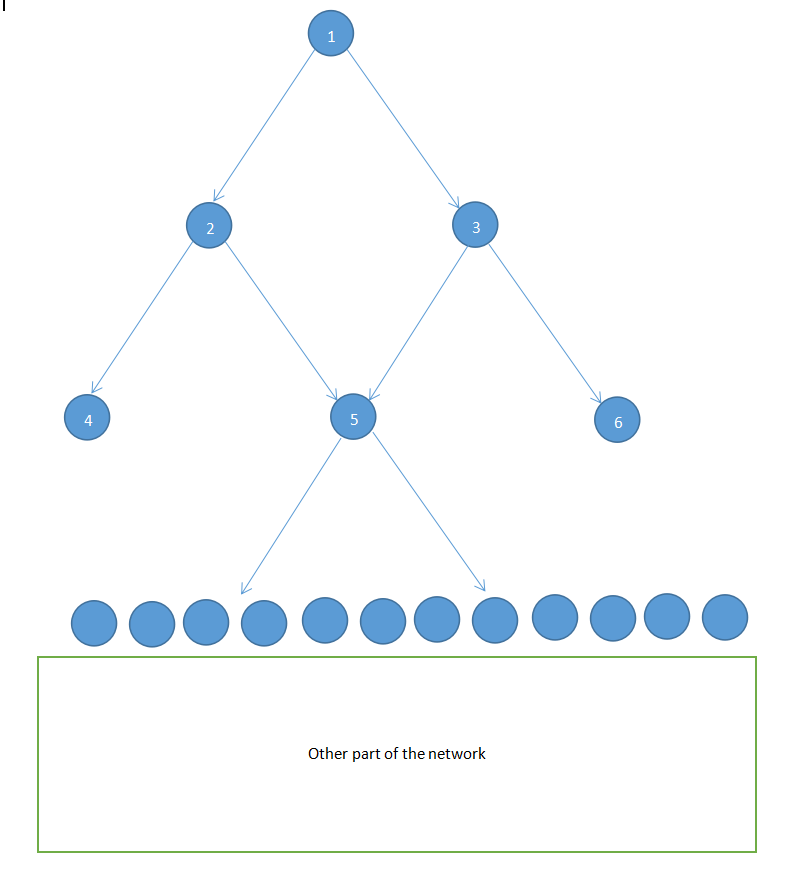
\includegraphics[width = 6cm]{1.png}
	\caption{Example network before removing $node_5$  }
	\label{fig:figure1}
	\end{figure}
	
	\begin{figure}[htp]
	\centering 
	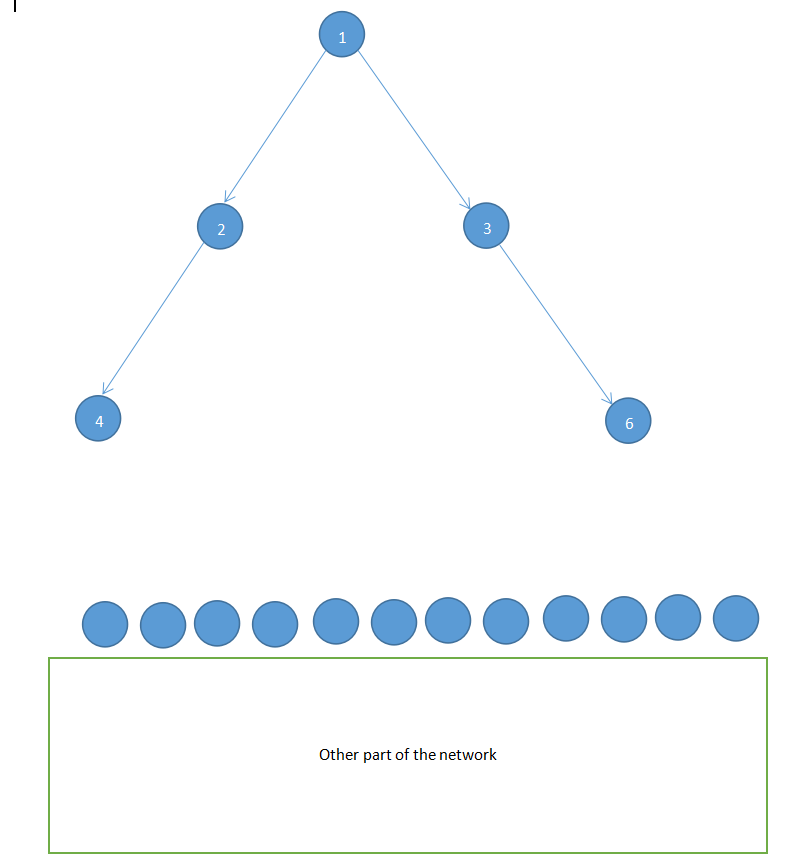
\includegraphics[width = 6cm]{2.png}
	\caption{Example network before after removing $node_5$  }
	\label{fig:figure2}
	\end{figure}	
	
	\subsection{Experiments on CI}				
	
	The following part of this section describes the experiments of CI on the ComplexCi and CI\_HEAP. Radius of 0,1,2 as input parameters in table \ref{tab:table6} and table \ref{tab:table7} are used to verify the performance on 8 competition datasets both for my C++ implementation ComplexCi and original c code CI\_HEAP. The \textit{minPoint} and \textit{algoEndsPoint} row are also involved into the result to evaluate the performance as brief reference. \textit{minPoint} means the number of removed nodes when ratio of giant component is invoking reinsertion on 1\%. \textit{algoEndsPoint} means the number of removed nodes when ratio of giant component is on 0. \textit{a.k.a.} there is no edge left in the network.
	
		
	
	\begin{table}[!htbp]
		\begin{adjustwidth}{-1cm}{}		
		\begin{threeparttable}		
		\centering
		\caption{Using ComplexCi to get robustness value, time, minPoint and algoEndsPoint on 8 competition datasets with reinsertion}
		\label{tab:table6}
		\begin{tabular}{|c|c|c|c|c|c|c|c|c|c|}
			\hline
			\textbf{Radius 0} & \textbf{model1} & \textbf{model2} & \textbf{model3} & \textbf{model4} & \textbf{real1} & \textbf{real2} & \textbf{real3} & \textbf{real4} & \textbf{total} \\ \hline
			Robustness score                   & 0.2130          & 0.1783          & 0.3488          & 0.1304          & 0.0459         & 0.0918         & 0.1030         & 0.0751         & 1.1863         \\ \hline
			time                    & 150s            & 117s            & 215s            & 92s             & 203s           & 90s            & 171s           & 148s           & 215s           \\ \hline
			minPoint                & 322306          & 281709          & 538703          & 200339          & 220297         & 508819         & 93807          & 171159         &                \\ \hline
			algoEndsPoint           & 583934          & 573704          & 719722          & 534504          & 529690         & 1054742        & 151903         & 343549         &                \\ \hline
			
			\textbf{Radius 1} & \textbf{model1} & \textbf{model2} & \textbf{model3} & \textbf{model4} & \textbf{real1} & \textbf{real2} & \textbf{real3} & \textbf{real4} & \textbf{total} \\ \hline
			Robustness score                            & 0.2079          & 0.1729          & 0.3459          & 0.1258          & 0.0407         & 0.0545         & 0.0969         & 0.0654         & 1.1099         \\ \hline
			time                             & 218s            & 176s            & 324s            & 138s            & 526s           & 62s            & 637s           & 170s           & 637s           \\ \hline
			minPoint                         & 301512          & 260039          & 528727          & 190322          & 186405         & 332689         & 85279          & 162601         &                \\ \hline
			algoEndsPoint                    & 675627          & 677816          & 779027          & 632197          & 718846         & 1293988        & 186872         & 430115         &                \\ \hline		
			
			\textbf{Radius 2} & \textbf{model1} & \textbf{model2} & \textbf{model3} & \textbf{model4} & \textbf{real1} & \textbf{real2} & \textbf{real3} & \textbf{real4} & \textbf{total} \\ \hline
			Robustness score                 & 0.2083          & 0.1732          & 0.3446          & 0.1189          & 0.0387         & 0.0417         & 0.0955         & 0.0492         & 1.0701         \\ \hline
			time                             & 1757s           & 716s            & 1734s           & 475s            & 27555s         & 57s            & 43181s         & 1005s          & 43181s         \\ \hline
			minPoint                         & 301512          & 260039          & 518751          & 170288          & 169459         & 254409         & 85279          & 171159         &                \\ \hline
			algoEndsPoint                    & 686650          & 695091          & 772235          & 690491          & 766671         & 1355969        & 189648         & 509904         &                \\ \hline
	
		\end{tabular}
		\begin{tablenotes}
			\small
			\item\textit{ 8 datasets are all verified in concurrent. The time doesn\textquotesingle t cover IO read/write from/to disk.}
		\end{tablenotes}			
		\end{threeparttable}
		\end{adjustwidth}	
	\end{table}
	
	
	\begin{table}[!htbp]
	\begin{adjustwidth}{-1cm}{}		
		\begin{threeparttable}		
			\centering
			\caption{Using CI\_HEAP to get robustness value, time, minPoint on 8 competition datasets with reinsertion}
			\label{tab:table7}
			\begin{tabular}{|c|c|c|c|c|c|c|c|c|c|}
				\hline
				\textbf{Radius 0} & \textbf{model1} & \textbf{model2} & \textbf{model3} & \textbf{model4} & \textbf{real1} & \textbf{real2} & \textbf{real3} & \textbf{real4} & \textbf{total} \\ \hline
				Robustness score                 & 0.2121          & 0.1771          & 0.3485          & 0.1286          & 0.0450         & 0.0903         & 0.1022         & 0.0755         & 1.1793         \\ \hline
				time                             & 184s            & 156s            & 307s            & 117s            & 708s           & 95s            & 498s           & 169s           & 708s           \\ \hline
				minPoint                         & 322308          & 281711          & 538705          & 200341          & 220299         & 430541         & 93809          & 171161         &                \\ \hline
				
				\textbf{Radius 1} & \textbf{model1} & \textbf{model2} & \textbf{model3} & \textbf{model4} & \textbf{real1} & \textbf{real2} & \textbf{real3} & \textbf{real4} & \textbf{total} \\ \hline
				Robustness score                 & 0.2080          & 0.1732          & 0.3460          & 0.1249          & 0.0410         & 0.0490         & 0.0964         & 0.0659         & 1.1045         \\ \hline
				time                             & 195s            & 159s            & 333s            & 119s            & 604s           & 68s            & 727s           & 179s           & 727s           \\ \hline
				minPoint                         & 301514          & 260041          & 528729          & 190324          & 186407         & 293551         & 89545          & 162603         &                \\ \hline
				
				\textbf{Radius 2} & \textbf{model1} & \textbf{model2} & \textbf{model3} & \textbf{model4} & \textbf{real1} & \textbf{real2} & \textbf{real3} & \textbf{real4} & \textbf{total} \\ \hline
				Robustness score                 & 0.2079&0.1732&0.3446&0.1189&0.0389&0.0418&0.0955&0.0489&1.0696         \\ \hline
				time                             &  1489s&503s&1417s&316s&30771s&57s&75332s&945s&75332s
				         \\ \hline
				minPoint                         & 301514&260041&518753&170290&169461&234841&85281&171161
				     &                \\ \hline				
			\end{tabular}
			\begin{tablenotes}
				\small
				\item\textit{ 8 datasets are all verified in concurrent. The time doesn\textquotesingle t cover IO read/write from/to disk.}
			\end{tablenotes}			
		\end{threeparttable}
		\end{adjustwidth}	
	\end{table}	
	
	It is also curious about the roles of reinsertion plays in the overall performance. What will performance of the result be if we remove the reinsertion in the algorithm of CI ? I also try to verify the case of disabling reinsertion. Results without reinsertion are shown in the table \ref{tab:table8} and table \ref{tab:table9} 
	
	\begin{table}[!htbp]
	\begin{adjustwidth}{-1cm}{}		
		\begin{threeparttable}		
			\centering
			\caption{Using ComplexCi to get robustness value, time, minPoint and algoEndsPoint  on 8 competition datasets without reinsertion}
			\label{tab:table8}
			\begin{tabular}{|c|c|c|c|c|c|c|c|c|c|}
				\hline
				\textbf{Radius 0} & \textbf{model1} & \textbf{model2} & \textbf{model3} & \textbf{model4} & \textbf{real1} & \textbf{real2} & \textbf{real3} & \textbf{real4} & \textbf{total} \\ \hline
				Robustness score                 & 0.2279          & 0.1914          & 0.3794          & 0.1446          & 0.0493         & 0.0689         & 0.1102         & 0.0922         & 1.2638         \\ \hline
				time                             & 21s             & 16s             & 20s             & 14s             & 20s            & 5s             & 19s            & 19s            & 20s            \\ \hline
				minPoint                & 322306          & 281709          & 538703          & 200339          & 220297         & 508819         & 93807          & 171159         &                \\ \hline
				algoEndsPoint           & 583934          & 573704          & 719722          & 534504          & 529690         & 1054742        & 151903         & 343549         &                \\ \hline
				
				\textbf{Radius 1} & \textbf{model1} & \textbf{model2} & \textbf{model3} & \textbf{model4} & \textbf{real1} & \textbf{real2} & \textbf{real3} & \textbf{real4} & \textbf{total} \\ \hline
				Robustness score                 & 0.2253          & 0.1878          & 0.3809          & 0.1434          & 0.0523         & 0.1069         & 0.1118         & 0.1024         & 1.3108         \\ \hline
				time                             & 115s            & 87s             & 134s            & 65s             & 359s           & 12s            & 470s           & 59s            & 470s           \\ \hline
				minPoint                         & 301512          & 260039          & 528727          & 190322          & 186405         & 332689         & 85279          & 162601         &                \\ \hline
				algoEndsPoint                    & 675627          & 677816          & 779027          & 632197          & 718846         & 1293988        & 186872         & 430115         &                \\ \hline		
				
				\textbf{Radius 2} & \textbf{model1} & \textbf{model2} & \textbf{model3} & \textbf{model4} & \textbf{real1} & \textbf{real2} & \textbf{real3} & \textbf{real4} & \textbf{total} \\ \hline
				Robustness score                 & 0.2239          & 0.1867          & 0.3777          & 0.1317          & 0.0482         & 0.0941         & 0.1085         & 0.0962         & 1.2671         \\ \hline
				time                             & 1717s           & 661s            & 1533s           & 441s            & 27250s         & 21s            & 43127s         & 907s           & 43127s         \\ \hline
				minPoint                         & 301512          & 260039          & 518751          & 170288          & 169459         & 254409         & 85279          & 171159         &                \\ \hline
				algoEndsPoint                    & 686650          & 695091          & 772235          & 690491          & 766671         & 1355969        & 189648         & 509904         &                \\ \hline
				
			\end{tabular}
			\begin{tablenotes}
				\small
				\item\textit{ 8 datasets are all verified in concurrent. The time doesn\textquotesingle t cover IO read/write from/to disk.}
				\end{tablenotes}			
			\end{threeparttable}
		\end{adjustwidth}	
	\end{table}
	
	
	\begin{table}[!htbp]
		\begin{adjustwidth}{-1cm}{}		
			\begin{threeparttable}		
				\centering
				\caption{Using CI\_HEAP to get robustness value, time, minPoint on 8 competition datasets without reinsertion}
				\label{tab:table9}
				\begin{tabular}{|c|c|c|c|c|c|c|c|c|c|}
					\hline
					\textbf{Radius 0} & \textbf{model1} & \textbf{model2} & \textbf{model3} & \textbf{model4} & \textbf{real1} & \textbf{real2} & \textbf{real3} & \textbf{real4} & \textbf{total} \\ \hline
					Robustness score                 & 0.2282          & 0.1916          & 0.3794          & 0.1438          & 0.0492         & 0.0773         & 0.1102         & 0.0927         & 1.2723         \\ \hline
					time                             & 18s             & 16s             & 24s             & 14s             & 22s            & 13s            & 21s            & 16s            & 22s            \\ \hline
					minPoint                         & 322308          & 281711          & 538705          & 200341          & 220299         & 430541         & 93809          & 171161         &                \\ \hline
					
					\textbf{Radius 1} & \textbf{model1} & \textbf{model2} & \textbf{model3} & \textbf{model4} & \textbf{real1} & \textbf{real2} & \textbf{real3} & \textbf{real4} & \textbf{total} \\ \hline
					Robustness score                 & 0.2254          & 0.1878          & 0.3811          & 0.1433          & 0.0533         & 0.1111         & 0.1119         & 0.1032         & 1.3170         \\ \hline
					time                             & 38s             & 27s             & 51s             & 20s             & 122s           & 12s            & 269s           & 27s            & 269s           \\ \hline
					minPoint                         & 301514          & 260041          & 528729          & 190324          & 186407         & 293551         & 89545          & 162603         &                \\ \hline
					
					\textbf{Radius 2} & \textbf{model1} & \textbf{model2} & \textbf{model3} & \textbf{model4} & \textbf{real1} & \textbf{real2} & \textbf{real3} & \textbf{real4} & \textbf{total} \\ \hline
					Robustness score                 & 0.2239          & 0.1867          & 0.3777          & 0.1317          & 0.0491         & 0.0966         & 0.1086         & 0.0965         & 1.2709         \\ \hline
					time                             & 1324s           & 384s            & 1141s           & 225s            & 30390s         & 15s            & 75070s         & 841s           & 75070s         \\ \hline
					minPoint                         & 301514          & 260041          & 518753          & 170290          & 169461         & 234841         & 85281          & 171161         &                \\ \hline				
				\end{tabular}
				\begin{tablenotes}
					\small
					\item\textit{ 8 datasets are all verified in concurrent. The time doesn\textquotesingle t cover IO read/write from/to disk.}
				\end{tablenotes}			
			\end{threeparttable}
		\end{adjustwidth}	
	\end{table}	



	In table \ref{tab:table10} and \ref{tab:table11}, the time of \textit{CI with reinsertion}, \textit{CI without reinsertion} and \textit{reinsertion excluding CI} are shown for ComplexCi and CI\_HEAP. \textit{reinsertion excluding CI} is calculated by \textit{CI with reinsertion} minus \textit{CI without reinsertion}

	\begin{table}[!htbp]
	\begin{adjustwidth}{-2cm}{}		
		\begin{threeparttable}		
			\centering
			\caption{Using ComplexCi to get time on 8 competition datasets, including CI with reinsertion, without reinsertion and reinsertion excluding CI}
			\label{tab:table10}
			\begin{tabular}{|c|c|c|c|c|c|c|c|c|c|}
				\hline
				\textbf{Radius 0} & \textbf{model1} & \textbf{model2} & \textbf{model3} & \textbf{model4} & \textbf{real1} & \textbf{real2} & \textbf{real3} & \textbf{real4} & \textbf{total} \\ \hline
				
				CI with reinsertion time                 & 150s&117s&215s&92s&203s&90s&171s&148s&215s         \\ \hline
				CI without reinsertion time                             & 21s&16s&20s&14s&20s&5s&19s&19s&20s            \\ \hline
				reinsertion time excluding CI                         & 129s&101s&195s&78s&183s&85s&152s&129s&195s               \\ \hline
				
				\textbf{Radius 1} & \textbf{model1} & \textbf{model2} & \textbf{model3} & \textbf{model4} & \textbf{real1} & \textbf{real2} & \textbf{real3} & \textbf{real4} & \textbf{total} \\ \hline
				
				CI with reinsertion time                 & 218s&176s&324s&138s&526s&62s&637s&170s&637s         \\ \hline
				CI without reinsertion time                             & 115s&87s&134s&65s&359s&12s&470s&59s&470s            \\ \hline
				reinsertion time excluding CI                         & 103s&89s&190s&73s&167s&50s&167s&111s&167s               \\ \hline					
				
				\textbf{Radius 2} & \textbf{model1} & \textbf{model2} & \textbf{model3} & \textbf{model4} & \textbf{real1} & \textbf{real2} & \textbf{real3} & \textbf{real4} & \textbf{total} \\ \hline
				CI with reinsertion time                 & 1757s&716s&1734s&475s&27555s&57s&43181s&1005s&43181s         \\ \hline
				CI without reinsertion time                             & 1717s&661s&1533s&441s&27250s&21s&43127s&907s&43127s         \\ \hline
				reinsertion time excluding CI                         & 40s&55s&201s&34s&305s&36s&54s&98s&54s                \\ \hline				
			\end{tabular}
			\begin{tablenotes}
				\small
				\item\textit{ 8 datasets are all verified in concurrent. The time doesn\textquotesingle t cover IO read/write from/to disk.}
			\end{tablenotes}			
		\end{threeparttable}
	\end{adjustwidth}	
	\end{table}	


	\begin{table}[!htbp]
	\begin{adjustwidth}{-2cm}{}		
		\begin{threeparttable}		
			\centering
			\caption{Using CI\_HEAP to get time on 8 competition datasets, including CI with reinsertion, without reinsertion and reinsertion excluding CI}
			\label{tab:table11}
			\begin{tabular}{|c|c|c|c|c|c|c|c|c|c|}
				\hline
				\textbf{Radius 0} & \textbf{model1} & \textbf{model2} & \textbf{model3} & \textbf{model4} & \textbf{real1} & \textbf{real2} & \textbf{real3} & \textbf{real4} & \textbf{total} \\ \hline
				
				CI with reinsertion time                 & 184s&156s&307s&117s&708s&95s&498s&169s&708s         \\ \hline
				CI without reinsertion time                             & 18s&16s&24s&14s&22s&13s&21s&16s&22s            \\ \hline
				reinsertion time excluding CI                         & 166s&140s&283s&103s&686s&82s&477s&153s&686s               \\ \hline
				
				\textbf{Radius 1} & \textbf{model1} & \textbf{model2} & \textbf{model3} & \textbf{model4} & \textbf{real1} & \textbf{real2} & \textbf{real3} & \textbf{real4} & \textbf{total} \\ \hline
				
				CI with reinsertion time                 & 195s&159s&333s&119s&604s&68s&727s&179s&727s         \\ \hline
				CI without reinsertion time                             & 38s&27s&51s&20s&122s&12s&269s&27s&269s            \\ \hline
				reinsertion time excluding CI                         & 157s&132s&282s&99s&482s&56s&458s&152s&458s               \\ \hline					
				
				\textbf{Radius 2} & \textbf{model1} & \textbf{model2} & \textbf{model3} & \textbf{model4} & \textbf{real1} & \textbf{real2} & \textbf{real3} & \textbf{real4} & \textbf{total} \\ \hline
				CI with reinsertion time                 & 1489s&503s&1417s&316s&30771s&57s&75332s&945s&75332s         \\ \hline
				CI without reinsertion time                             & 1324s&384s&1141s&225s&30390s&15s&75070s&841s&75070s         \\ \hline
				reinsertion time excluding CI                         & 165s&119s&276s&91s&381s&42s&262s&104s&262s                \\ \hline				
			\end{tabular}
			\begin{tablenotes}
				\small
				\item\textit{ 8 datasets are all verified in concurrent. The time doesn\textquotesingle t cover IO read/write from/to disk.}
			\end{tablenotes}			
		\end{threeparttable}
	\end{adjustwidth}	
	\end{table}	

	
	From the experiments in table \ref{tab:table6}, \ref{tab:table7}, \ref{tab:table8}, \ref{tab:table9}, \ref{tab:table10}, \ref{tab:table11} , we can observe that:
	
	\begin{enumerate}
		
		
	\begin{item}
		CI in higher radius parameter performs better than Betweenness, Closeness, PageRank and Degree
	\end{item}		
		
		\begin{item}
			ComplexCi and CI\_HEAP are able to get the nearly same result in the same internal parameter. But there is still slightly different between them. I think it may be caused by the following reasons:
			
			\begin{enumerate}
				\begin{item}
					When CI removes the nodes one by one, there is the possibility that at least 2 nodes get the same CI value. CI will treat the same score nodes as the equality and choose one random node to delete. So CI depends heavily on the order of the removed node. The different deletion choice for the same score node will lead to the different robustness values finally. 
				\end{item}
				\begin{item}
					When reinsertion adds back the node one by one or a finite fraction of nodes in the batch operation, it will also meet with the same score for several nodes, which is similar with the above situation. Reinsertion will add back nodes of the same score randomly. Different reinsertion choice for the same score node will lead to the different robustness values finally as well.
				\end{item}		
				\begin{item}
					CI\_HEAP stops running algorithm when reaching \textit{minPoint} 0.01. ComplexCi will continue to run until reaching \textit{algoEndsPoint}, which represents that there is no edge in the network
				\end{item}			
				
			\end{enumerate}			
			
			
		\end{item}			
		
		\begin{item}
			Consuming time is increasing according to the higher ball radius in both ComplexCi and CI\_HEAP. After debugging and profiling, I find that most time-consuming section is to find the nodes in the scope of defined radius by using breadth-first-search (BFS) algorithm. We can not ignore BFS complexity if ball radius is high. It is also interesting that running time of CI algorithm is not related with the node number. The largest network real2 performs the quickest to accomplish among all datasets and the smallest real3 performs the slowest as the radius 2.
		\end{item}

	
		\begin{item}
			ComplexCI can get better speed than CI\_HEAP without reinsertion in high radius. For the real1 and real3, it can even reduce the spent time in 50\% when radius is 2. I believe the main cause is the implementation of the breadth-first-search (BFS) algorithm because it is the most time-consuming method in CI algorithm after profiling and debugging the code, though I didn\textquotesingle t get the detailed experiment statistic on it. 	
		\end{item}	
	
		\begin{item}	
			In table \ref{tab:table10} and table \ref{tab:table11}, \textit{reinsertion time excluding CI} become shorter according to the higher radius parameter since it will reach the start of reinsertion process earlier. We can also see that ComplexCI is better in speed in the process of reinsertion excluding running CI. It is the evidence that using disjoint-set strategy in ComplexCi performs more efficiently than original reinsertion algorithm in CI\_HEAP. 
		\end{item}	
	
		\begin{item}	
			Although the \textit{minPoint} reaches 0.01 and \textit{algoEndsPoint} reaches 0 of giant graph connected component ratio earlier in the higher radius, it seems that CI performs worse in terms of robustness value without reinsertion. I regard CI is just able to deal with controlling minimum number of nodes leading to the collapsed network, but CI is not good at getting better robustness value . So from this observation we are curious that whether the CI just works because of the reinsertion. Or can we develop the better reinsertion algorithm without using CI in robustness ? I will elaborate my thinking and experiments on that in the next chapter.	
		\end{item}		
		
	\end{enumerate}
			

	\section{New Reinsertion algorithm}

	\subsection{Join the clusters of smallest sizes}

	Let\textquotesingle s back to see the above description of reinsertion
	
	\begin{itquote}
	
	Reinsertion adds back one of the removed nodes, which is chosen such that, if once reinserted, it joins the smallest number of clusters. Reinsertion algorithm does not require that the reinserted node joins the clusters of smallest sizes, but only the minimum number of clusters, independently from their sizes. When the node is reinserted reinsertion also restores the edges with its neighbors which are in the network (but not the ones with neighbors not yet reinserted, if any). The procedure is repeated until all the nodes are back in the network. 
	
	\end{itquote}	
	
	 It is strange that the author of \cite{morone2015influence} \cite{morone2016collective} say "reinsertion algorithm does not require that the reinserted node joins the clusters of smallest sizes, but only the minimum number of clusters, independently from their sizes.". I can not guess why they use the minimum number of clusters. In fact, I tend to believe that the reinserted node joining the clusters of smallest sizes will get better robustness value instead of the one joining only minimum number of clusters. The experiments of modified reinsertion joining the clusters of smallest sizes are shown in the table \ref{tab:table12}. For the convenience, I call the algorithm of modified reinsertion joining the clusters of smallest sizes as \textit{New-Reinsertion}, and the algorithm of traditional reinsertion joining the minimum number of clusters as \textit{Traditional-Reinsertion} in the following paper.
	 
	 
	\begin{table}[!htbp]
	\begin{adjustwidth}{-1cm}{}		
		\begin{threeparttable}		
			\centering
			\caption{Using CI with modified reinsertion joining the clusters of smallest sizes (\textit{New-Reinsertion}) to get robustness value, time, minPoint and algoEndsPoint  on 8 competition datasets}
			\label{tab:table12}
			\begin{tabular}{|c|c|c|c|c|c|c|c|c|c|}
				\hline
				\textbf{Radius 0} & \textbf{model1} & \textbf{model2} & \textbf{model3} & \textbf{model4} & \textbf{real1} & \textbf{real2} & \textbf{real3} & \textbf{real4} & \textbf{total} \\ \hline
				Robustness score                 & 0.2100    & 0.1744    & 0.3603    & 0.1175    & 0.0315    & 0.0069    & 0.0978    & 0.0417    & 1.0403    \\ \hline
				
				time                             & 148s      & 126s      & 211s      & 95s       & 163s      & 103s      & 161s      & 137s      & 211s      \\ \hline
				minPoint                & 322306          & 281709          & 538703          & 200339          & 220297         & 508819         & 93807          & 171159         &                \\ \hline
				algoEndsPoint           & 583934          & 573704          & 719722          & 534504          & 529690         & 1054742        & 151903         & 343549         &                \\ \hline
				
				\textbf{Radius 1} & \textbf{model1} & \textbf{model2} & \textbf{model3} & \textbf{model4} & \textbf{real1} & \textbf{real2} & \textbf{real3} & \textbf{real4} & \textbf{total} \\ \hline
				Robustness score                 & 0.2104    & 0.1743    & 0.3656    & 0.1152    & 0.0318    & 0.0046    & 0.0968    & 0.0421    & 1.0409    \\ \hline
				
				time                             & 219s      & 177s      & 317s      & 135s      & 487s      & 65s       & 630s      & 163s      & 630s      \\ \hline
				
				minPoint                         & 301512          & 260039          & 528727          & 190322          & 186405         & 332689         & 85279          & 162601         &                \\ \hline
				algoEndsPoint                    & 675627          & 677816          & 779027          & 632197          & 718846         & 1293988        & 186872         & 430115         &                \\ \hline		
				
				\textbf{Radius 2} & \textbf{model1} & \textbf{model2} & \textbf{model3} & \textbf{model4} & \textbf{real1} & \textbf{real2} & \textbf{real3} & \textbf{real4} & \textbf{total} \\ \hline
				Robustness score                 & 0.2107    & 0.1739    & 0.3585    & 0.1148    & 0.0303    & 0.0039    & 0.0954    & 0.0370    & 1.0246    \\ \hline
				
				time                             & 1767s     & 716s      & 1715s     & 478s      & 27488s    & 58s       & 43224s    & 1044s     & 43224s    \\ \hline
				
				minPoint                         & 301512          & 260039          & 518751          & 170288          & 169459         & 254409         & 85279          & 171159         &                \\ \hline
				algoEndsPoint                    & 686650          & 695091          & 772235          & 690491          & 766671         & 1355969        & 189648         & 509904         &                \\ \hline
				
			\end{tabular}
			\begin{tablenotes}
				\small
				\item\textit{ 8 datasets are all verified in concurrent. The time doesn\textquotesingle t cover IO read/write from/to disk.}
			\end{tablenotes}			
		\end{threeparttable}
	\end{adjustwidth}	
	\end{table}
	 
	 
	 When implementing the algorithm of modified reinsertion joining the clusters of smallest sizes \textit{New-Reinsertion}, I just use nearly the same algorithm \ref{algo:algo1} by disjoint-set data structure mentioned above. The only difference from algorithm \ref{algo:algo1} is that the reinsertion joining clusters of smallest sizes \textit{New-Reinsertion} is used. Since the \textit{Rank} technique is used to optimize the performance of disjoint-set data structure, size information for each cluster is stored in the disjoint-set \textit{Rank} array, which can be easy to be picked up for determining the smallest one. With the help of disjoint-set data structure, fetching size for each cluster will be only $O(inverse\_aka(n))$ and nearly constant time. Algorithm of \textit{New-Reinsertion} are shown in algorithm \ref{algo:algo2} and codes are based on the ComplexCi
	 
	\begin{algorithm}[!htbp]
	\caption{ The algorithm of modified reinsertion joining the clusters of smallest sizes \textit{New-Reinsertion} }
	\label{algo:algo2}
	\begin{algorithmic}[1]
		\State We have the initial collapsed complex network and build the corresponding disjoint-set data structure.
		
		\State Then choose the left nodes to reconstruct the network:
		
		\begin{algsubstates}
			\State For each left $node_i$ , if once reinserted, \textit{Find} operation will be used to select the connected component indices of neighborhoods nodes around node i one by one in the disjoint-set data structure, which is named as $C_{i1}$, $C_{i2}$ ... , $C_{in}$. 
			
			\State Then we need to check whether there are the duplicated connected component indices in the set $C_i$ and make item in the set $C_i$ to be unique. The new unique set will be $UC_{i1}$, $UC_{i2}$ ... , $UC_{im}$.  
			
			\State Get the connected component size information $rank[UC_{i}]$ from \textit{rank} array due to the fact that each cluster size is stored in it. Sum up all $rank[UC_{i1}]$, $rank[UC_{i2}]$, ... $rank[UC_{im}]$ as $S_i$ to get the clusters sizes which will be joined if the $node_i$ is reinserted.
			
			\State Search for the smallest $S_{min}$ value of $Node_{min}$ among all left nodes value $S_i$. We will reinsert the corresponding $Node_{min}$ into the network by the \textit{Union} operation, which will update the connected component indices information in the disjoint-set data structure. As mentioned above, when implementing the reinsertion,  the finite fraction of nodes are added back at each step.
			
			\State Repeat to search for the next reinsert node in step 2 until all left nodes are consumed.
		\end{algsubstates}
	\end{algorithmic}
	\end{algorithm}
	 
	
	The only difference of algorithm \ref{algo:algo1} and algorithm \ref{algo:algo2} is Step 2c. Although algorithm \ref{algo:algo1} and algorithm \ref{algo:algo2} are using different ways but their intentions both are getting the score which can represent the $node_i$. We can replace the Step 2c with the calculation kernel as more generic framework in algorithm \ref{algo:algo3}. Therefore, algorithm \ref{algo:algo3} is extracted as general ways to describe the process of reinsertion. It is certain that different kernel will lead to different behaviour in reinsertion combining with generic reinsertion framework. Algorithm \ref{algo:algo3} + algorithm \ref{algo:algo4} will get algorithm \ref{algo:algo1} as \textit{Traditional-Reinsertion}. Algorithm \ref{algo:algo3} + algorithm \ref{algo:algo5} will get algorithm \ref{algo:algo2} as \textit{New-Reinsertion}. 
	
	
	\begin{algorithm}[!htbp]
	\caption{ The algorithm of reinsertion with the calculation kernel in more generic framework: Generic reinsertion framework (GRF) }
	\label{algo:algo3}
	\begin{algorithmic}[1]
		\State We have the initial collapsed complex network and build the corresponding disjoint-set data structure.
		
		\State Then choose the left nodes to reconstruct the network:
		
		\begin{algsubstates}
			\State For each left $node_i$ , if once reinserted, \textit{Find} operation will be used to select the connected component indices of neighborhoods nodes around node i one by one in the disjoint-set data structure, which is named as $C_{i1}$, $C_{i2}$ ... , $C_{in}$. 
			
			\State Then we need to check whether there are the duplicated connected component indices in the set $C_i$ and make item in the set $C_i$ to be unique. The new unique set will be $UC_{i1}$, $UC_{i2}$ ... , $UC_{im}$.  
			
			\State Getting the score $J_i$ by specific calculation kernel which can represent the $node_i$.
			
			\State Search for the smallest $J_{min}$ value of $Node_{min}$ among all left nodes value $J_i$. We will reinsert the corresponding $Node_{min}$ into the network by the \textit{Union} operation, which will update the connected component indices information in the disjoint-set data structure. As mentioned above, when implementing the reinsertion,  the finite fraction of nodes are added back at each step.
			
			\State Repeat to search for the next reinsert node in step 2 until all left nodes are consumed.
		\end{algsubstates}
	\end{algorithmic}
	\end{algorithm}	




	\begin{algorithm}[!htbp]
		\caption{ \textit{Traditional-Reinsertion} kernel to get the score $J_i$ representing the $node_i$. }
		\label{algo:algo4}
		\begin{algorithmic}[1]
			\State Get the count of set $UC_{i}$ as $M_i$.
			\State return $M_i$ as $J_i$ 
		\end{algorithmic}
	\end{algorithm}	

	\begin{algorithm}[!htbp]
		\caption{ \textit{New-Reinsertion} kernel to get the score $J_i$ representing the $node_i$. }
		\label{algo:algo5}
		\begin{algorithmic}[1]
			\State Get the connected component size information $rank[UC_{i}]$ from \textit{rank} array due to the fact that each cluster size is stored in it. Sum up all $rank[UC_{i1}]$, $rank[UC_{i2}]$, ... $rank[UC_{im}]$ as $S_i$ to get the clusters sizes which will be joined if the $node_i$ is reinserted.
			\State return $S_i$ as $J_i$ 
		\end{algorithmic}
	\end{algorithm}	

	
	
	
	 In table \ref{tab:table12}, we can see that the total robustness score of \textit{New-Reinsertion} in radius 2 is better than any of the previous mentioned algorithm. Even the case when radius is 0 and CI degenerate to HDA is able to get the pretty better result 1.0403 in 4 minutes compared with previous best result 1.0701 in nearly 12 hours with \textit{Traditional-Reinsertion}. It means reinsertion plays more important role than CI for getting better robustness , though CI in higher radius with \textit{New-Reinsertion} can still help to improve the result and achieve the best score.
	 
	 
	 
	\subsection{For the better result}
	 

	In order to get better robustness score and high rank on the leaderboard of competition, more strict internal parameters are used. In detail , there are 2 internal parameters \textit{computeComponentInterval} and \textit{reinsertEachStep} changed here.
		
	\begin{enumerate}
		\begin{item}
			\textit{computeComponentInterval}: It means the interval to calculate giant component when complex network collapses. The original is 1 percent of the size of complete network. For the more strict parameter , the value is re-scaled to 200 if the original is larger than 200. It will revoke the start of reinsertion at certain value more precisely.
		\end{item}
		\begin{item}
			\textit{reinsertEachStep}: It means the batch size of nodes reinserted into the network per updating the graph. The original is 1 per mille of the size of complete network. For the more strict parameter , the value is re-scaled to 20 if the original is larger than 20, which will decrease the number of reinserted nodes at each reinsertion step.
		\end{item}		
		
	\end{enumerate}			
		
	The \textit{Str-New-Reinsertion} and \textit{Str-Trad-Reinsertion} in radius 2 are shown in the table \ref{tab:table13} after applying more strict internal parameters \textit{computeComponentInterval} and \textit{reinsertEachStep}. Compared with \textit{New-Reinsertion} and \textit{Trad-Reinsertion}, the less interval of \textit{computeComponentInterval} and \textit{reinsertEachStep} will bring benefit to the better total robustness. For most each provided datasets, \textit{Str-New-Reinsertion} will get the better result but the only exception is the network model3. The better scores of \textit{Str-New-Reinsertion} and \textit{Str-Trad-Reinsertion} are organized as selective score shown at the bottom of table \ref{tab:table13}.
	 
	 
	\begin{table}[!htbp]
	\begin{adjustwidth}{-2cm}{}		
		\begin{threeparttable}		
			\centering
			\caption{Using CI in radius 2 of \textit{Str-New-Reinsertion} and \textit{Str-Trad-Reinsertion}  after applying more strict internal parameters to get robustness value, time, minPoint and algoEndsPoint on 8 competition datasets}
			\label{tab:table13}
			\begin{tabular}{|c|c|c|c|c|c|c|c|c|c|}
				\hline
					
				\textbf{Str-Trad-Reinsertion} & \textbf{model1} & \textbf{model2} & \textbf{model3} & \textbf{model4} & \textbf{real1} & \textbf{real2} & \textbf{real3} & \textbf{real4} & \textbf{total} \\ \hline
				Robustness score                 & 0.2074          & 0.1725          & \textbf{0.3441}          & 0.1193          & 0.0384         & 0.0392         & 0.0956         & 0.0497         & 1.0662         \\ \hline
				time                             & 6469s           & 4762s           & 10320s          & 2993s           & 35680s         & 2657s          & 46928s         & 4772s          & 46928s         \\ \hline
				minPoint                         & 291599          & 251399          & 517999          & 163199          & 165799         & 242599         & 81199          & 162999         &                \\ \hline
				algoEndsPoint                    & 686650          & 695091          & 772235          & 690491          & 766671         & 1355969        & 189648         & 509904         &                \\ \hline
				\textbf{Str-New-Reinsertion}         & \textbf{model1} & \textbf{model2} & \textbf{model3} & \textbf{model4} & \textbf{real1} & \textbf{real2} & \textbf{real3} & \textbf{real4} & \textbf{total} \\ \hline
				Robustness score                 & \textbf{0.2072}          & \textbf{0.1710}          & 0.3596          & \textbf{0.1122}          & \textbf{0.0289}         & \textbf{0.0042}         & \textbf{0.0953}         & \textbf{0.0365}         & 1.0148         \\ \hline
				time                             & 6529s           & 4823s           & 9874s           & 2953s           & 33599s         & 2728s          & 46701s         & 4807s          & 46701s         \\ \hline
				minPoint                         & 291599          & 251399          & 517999          & 163199          & 165799         & 242599         & 81199          & 162999         &                \\ \hline
				algoEndsPoint                    & 686650          & 695091          & 772235          & 690491          & 766671         & 1355969        & 189648         & 509904         &           \\ \hline \hline  
				\textbf{Selective Score}                 & \textbf{0.2072}          & \textbf{0.1710}          & \textbf{0.3441}          & \textbf{0.1122}          & \textbf{0.0289}         & \textbf{0.0042}         & \textbf{0.0953}         & \textbf{0.0365}         & \textbf{0.9993}   \\ \hline 				

			\end{tabular}
			\begin{tablenotes}
				\small
				\item\textit{ 8 datasets are all verified in concurrent. The time doesn\textquotesingle t cover IO read/write from/to disk.}
			\end{tablenotes}			
		\end{threeparttable}
	\end{adjustwidth}	
	\end{table}
	 
	Other enhanced reinsertion algorithms are also tried to get the better score.
	 
	\begin{enumerate}
		
	\begin{item}
			
		\textit{multiply-Reinsertion}: There have already been 2 calculation kernels proposed above, \textit{Traditional-Reinsertion} kernel in algorithm \ref{algo:algo4} and \textit{New-Reinsertion} kernel in algorithm \ref{algo:algo5}. Here the new \textit{multiply-Reinsertion} is designed in algorithm \ref{algo:algo6} , which multiplies $M_i$ of \textit{Traditional-Reinsertion} by $S_i$ of \textit{New-Reinsertion}. Since model3 is the only network dataset rejecting the better performance in \textit{New-Reinsertion}, I would like to adopt the combination of \textit{New-Reinsertion} and \textit{Traditional-Reinsertion} to see whether it will be more general to all datasets.

		\begin{algorithm}[!htbp]
			\caption{ \textit{multiply-Reinsertion} to get the score $J_i$ representing the $node_i$. }
			\label{algo:algo6}
			\begin{algorithmic}[1]
				\State Get the connected component size information $rank[UC_{i}]$ from \textit{rank} array due to the fact that each cluster size is stored in it. Sum up all $rank[UC_{i1}]$, $rank[UC_{i2}]$, ... $rank[UC_{im}]$ as $S_i$ to get the clusters sizes which will be joined if the $node_i$ is reinserted.
				\State Get the count of set $UC_{i}$ as $M_i$.			
				\State return $S_i*M_i$ as $J_i$ 
			\end{algorithmic}
		\end{algorithm}	
		
		In table \ref{tab:table14}, \textit{str-multiply-Reinsertion} with strict internal parameters of \textit{multiply-Reinsertion} shows that , though it will get total score 1.0115 better than \textit{Str-New-Reinsertion} 1.0148, the model3 network is still nearly the same and no further progress as in the \textit{Str-Traditional-Reinsertion}. Selective value in choosing better score of \textit{Str-Traditional-Reinsertion} and \textit{str-multiply-Reinsertion} is 0.9972 and it is just slightly better than 0.9993 in \ref{tab:table13}

	\end{item}
		
	\begin{item}
		\textit{lowerImportanceFirst}: When reinsertion adds back the node one by one or a finite fraction of nodes in the batch operation, it will meet with the same score for several nodes. Reinsertion will add back nodes of the same score randomly. For the strategy \textit{lowerImportanceFirst}, it chooses the nodes which are the same score ranking behind in the sequence of node importance with high priority when we apply reinsertion. a.k.a. Reinsert the node of the same score according to the order before reinsertion as much as possible. Here the score of $node_i$ refers to the $J_i$ in generic framework (GRF) algorithm \ref{algo:algo3}. However, the experiments of \textit{Str-LOW-MULTI-TRAD-Score} in the table \ref{tab:table14} with \textit{lowerImportanceFirst} on \textit{Selective Score} show that this heuristic idea is not obvious in the performance. In fact, it is nearly no use. I think it may caused that the same score for several nodes are not common in the reinsertion process.
	\end{item}
	\end{enumerate}	
	
		\begin{table}[!htbp]
		\begin{adjustwidth}{-3cm}{}		
		\begin{threeparttable}		
			\centering
			\caption{Using CI in radius 2 of \textit{multiply-Reinsertion} after applying more strict internal parameters to get robustness value, time, minPoint and algoEndsPoint on 8 competition datasets , compared with \textit{Str-Trad-Reinsertion}. Statistic of \textit{Str-LOW-MULTI-TRAD-Score} is applied with \textit{lowerImportanceFirst} on \textit{Selective Score} }
			\label{tab:table14}
			\begin{tabular}{|c|c|c|c|c|c|c|c|c|c|}
				\hline		
				
				
				\textbf{Str-Trad-Reinsertion} & \textbf{model1} & \textbf{model2} & \textbf{model3} & \textbf{model4} & \textbf{real1} & \textbf{real2} & \textbf{real3} & \textbf{real4} & \textbf{total} \\ \hline
				Robustness score                 & 0.2074          & 0.1725          & \textbf{0.3441}          & 0.1193          & 0.0384         & 0.0392         & 0.0956         & 0.0497         & 1.0662         \\ \hline
				time                             & 6469s           & 4762s           & 10320s          & 2993s           & 35680s         & 2657s          & 46928s         & 4772s          & 46928s         \\ \hline
				minPoint                         & 291599          & 251399          & 517999          & 163199          & 165799         & 242599         & 81199          & 162999         &                \\ \hline
				algoEndsPoint                    & 686650          & 695091          & 772235          & 690491          & 766671         & 1355969        & 189648         & 509904         &                \\ \hline
				
				\textbf{Str-multiply-Reinsertion}         & \textbf{model1} & \textbf{model2} & \textbf{model3} & \textbf{model4} & \textbf{real1} & \textbf{real2} & \textbf{real3} & \textbf{real4} & \textbf{total} \\ \hline
				Robustness score                 & \textbf{0.2060}&\textbf{0.1700}&0.3585&\textbf{0.1115}&\textbf{0.0310}&\textbf{0.0040}&\textbf{0.0939}&\textbf{0.0367}&1.0115         \\ \hline
				time                             & 6545s&4825s&9818s&2970s&34518s&2662s&46859s&4871s&46859s         \\ \hline
				minPoint                         & 291599          & 251399          & 517999          & 163199          & 165799         & 242599         & 81199          & 162999         &                \\ \hline
				algoEndsPoint                    & 686650          & 695091          & 772235          & 690491          & 766671         & 1355969        & 189648         & 509904         &           \\ \hline \hline  
				\textbf{Selective Score}                 & \textbf{0.2060}&\textbf{0.1700}&\textbf{0.3441}&\textbf{0.1115}&\textbf{0.0310}&\textbf{0.0040}&\textbf{0.0939}&\textbf{0.0367}&\textbf{0.9972}    \\ \hline 			
				\tabincell{c}{\textbf{Str-LOW-MULTI-TRAD-Score} \\  (lowerImportanceFirst \\ on Selective Score)}                 & \textbf{0.2063}&\textbf{0.1700}&\textbf{0.3442}&\textbf{0.1115}&\textbf{0.0307}&\textbf{0.0036}&\textbf{0.0940}&\textbf{0.0368}&\textbf{0.9972}   \\ \hline 						
				
			\end{tabular}
			\begin{tablenotes}
				\small
				\item\textit{ 8 datasets are all verified in concurrent. The time doesn\textquotesingle t cover IO read/write from/to disk.}
			\end{tablenotes}			
		\end{threeparttable}
	\end{adjustwidth}	
	\end{table}			
		
	 Currently we get the outstanding \textit{Str-LOW-MULTI-TRAD-Score} 0.9972 in table \ref{tab:table14}, which utilizes the techniques described in the algorithm \ref{algo:algo7}

		\begin{algorithm}[!htbp]
			\caption{ Summary of algorithms used in \textit{Str-LOW-MULTI-TRAD-Score} }
			\label{algo:algo7}
			\begin{algorithmic}[1]
				\State Collective Influence in radius 2.
				
				\State Generic reinsertion framework (GRF) in algorithm \ref{algo:algo3}.
				
				\State Model3 using \textit{Trad-Reinsertion} kernel in algorithm \ref{algo:algo4} with strict internal parameters \textit{Str-Trad-Reinsertion}
				
				\State All the other datasets except Model3 using \textit{multiply-Reinsertion} kernel in algorithm \ref{algo:algo6}  with strict internal parameters \textit{str-multiply-Reinsertion}
				
				\State Strategy \textit{lowerImportanceFirst}
				
				
			\end{algorithmic}
		\end{algorithm}


	 
	 \subsection{Tune parameters}
	 
	 
	 Next we need to tune input parameters to see whether we can get the better result. Different parameters will lead to different robustness value finally. There are 2 adjustable numeric input parameters in ComplexCi, including \textit{biggestComponentEndThreshold} and \textit{updateBatch}. 
	 	 
	\begin{enumerate}
	
		\begin{item}	
			\textit{biggestComponentEndThreshold}: Complex network collapses to the certain giant component ratio where the reinsertion algorithm starts in the generic reinsertion framework (GRF). The current default \textit{biggestComponentEndThreshold} for \textit{Str-LOW-MULTI-TRAD-Score} is 0.01. If users set it to zero, it means reinsertion will start until there is no edge in the network in removal.
		\end{item}
		
		\begin{item}	
			\textit{updateBatch}: Batch size of deleted points per updating Collective Influence value. Users can determine the batch size of deleting nodes in ComplexCi per updating CI values when the Complex Network collapses. The current default \textit{updateBatch} for \textit{Str-LOW-MULTI-TRAD-Score} is 1, which means that CI removes one node after updating CI values. It can be larger values and consumed time will be reduced.
		\end{item}	

	\end{enumerate}	
	 
	The concept similar with Grid Search \cite{wikiHyperparameter} is used to tune the parameters. The formal way of Grid Search is to find the best parameters in the subset of Cartesian product space of 2 sets \textit{biggestComponentEndThreshold} and \textit{updateBatch}. Here I just determine which \textit{biggestComponentEndThreshold} is suitable first , and then enlarge \textit{updateBatch} to see whether the rough updating will have negative impact on the robustness. Table \ref{tab:table15} shows the result of different \textit{biggestComponentEndThreshold} values in 0.0, 0.0001, 0.001, 0.01 and 0.1 on strategy \textit{Str-LOW-MULTI-TRAD-Score} and 0.001 is the best result among all. 
	
	\begin{table}[!htbp]
	\begin{adjustwidth}{-3cm}{}		
		\begin{threeparttable}		
			\centering
			\caption{Different \textit{biggestComponentEndThreshold} values in 0.0, 0.0001, 0.001, 0.01 and 0.1 on strategy \textit{Str-LOW-MULTI-TRAD-Score} to get robustness value, time, minPoint and algoEndsPoint on 8 competition datasets }
			\label{tab:table15}
			\begin{tabular}{|c|c|c|c|c|c|c|c|c|c|}
				\hline		
				
				
				\tabincell{c}{\textbf{Str-LOW-MULTI-TRAD-Score}\\ \textbf{with 0.0}} & \textbf{model1} & \textbf{model2} & \textbf{model3} & \textbf{model4} & \textbf{real1} & \textbf{real2} & \textbf{real3} & \textbf{real4} & \textbf{total} \\ \hline
				
				Robustness score & 0.2062          & 0.1698          & 0.3488          & 0.1101          & 0.0307         & 0.0021         & 0.0942         & 0.0404         & 1.0024         \\ \hline
				time             & 35310s          & 33122s          & 34847s          & 30200s          & 83939s         & 53483s         & 67617s         & 27982s         & 83939s         \\ \hline
				minPoint         & 686650          & 695091          & 772235          & 690491          & 766671         & 1355969        & 189648         & 509904         &                \\ \hline
				algoEndsPoint    & 686650          & 695091          & 772235          & 690491          & 766671         & 1355969        & 189648         & 509904         &                \\ \hline
				\tabincell{c}{\textbf{Str-LOW-MULTI-TRAD-Score}\\ \textbf{with 0.0001}}        & \textbf{model1} & \textbf{model2} & \textbf{model3} & \textbf{model4} & \textbf{real1} & \textbf{real2} & \textbf{real3} & \textbf{real4} & \textbf{total} \\ \hline
				Robustness score & 0.2057          & 0.1696          & 0.3441          & 0.1100          & 0.0307         & 0.0026         & 0.0936         & 0.0371         & 0.9934         \\ \hline
				time             & 9298s           & 6634s           & 13625s          & 4395s           & 63645s         & 6135s          & 50818s         & 15119s         & 63645s         \\ \hline
				minPoint         & 313599          & 273199          & 532399          & 193999          & 697999         & 341799         & 112399         & 469199         &                \\ \hline
				algoEndsPoint    & 686650          & 695091          & 772235          & 690491          & 766671         & 1355969        & 189648         & 509904         &                \\ \hline
				\tabincell{c}{\textbf{Str-LOW-MULTI-TRAD-Score}\\ \textbf{with 0.001}}  &\textbf{model1} & \textbf{model2} & \textbf{model3} & \textbf{model4} & \textbf{real1} & \textbf{real2} & \textbf{real3} & \textbf{real4} & \textbf{total} \\ \hline
				Robustness score & 0.2061          & 0.1699          & 0.3440          & 0.1107          & 0.0306         & 0.0026         & 0.0935         & 0.0358         & 0.9932         \\ \hline
				time             & 7565s           & 5640s           & 11772s          & 3533s           & 36134s         & 4113s          & 47758s         & 5868s          & 47758s         \\ \hline
				minPoint         & 296999          & 256399          & 520999          & 170199          & 183999         & 279399         & 83399          & 180799         &                \\ \hline
				algoEndsPoint    & 686650          & 695091          & 772235          & 690491          & 766671         & 1355969        & 189648         & 509904         &                \\ \hline
				\tabincell{c}{\textbf{Str-LOW-MULTI-TRAD-Score}\\ \textbf{with 0.01}} &\textbf{model1} & \textbf{model2} & \textbf{model3} & \textbf{model4} & \textbf{real1} & \textbf{real2} & \textbf{real3} & \textbf{real4} & \textbf{total} \\ \hline
				Robustness score & 0.2063          & 0.1700          & 0.3442          & 0.1115          & 0.0307         & 0.0036         & 0.0940         & 0.0368         & 0.9972         \\ \hline
				time             & 7015s           & 5156s           & 11236s          & 3176s           & 34970s         & 2922s          & 47242s         & 5052s          & 47242s         \\ \hline
				minPoint         & 291599          & 251399          & 517999          & 163199          & 165799         & 242599         & 81199          & 162999         &                \\ \hline
				algoEndsPoint    & 686650          & 695091          & 772235          & 690491          & 766671         & 1355969        & 189648         & 509904         &                \\ \hline
				\tabincell{c}{\textbf{Str-LOW-MULTI-TRAD-Score}\\ \textbf{with 0.1}} & \textbf{model1} & \textbf{model2} & \textbf{model3} & \textbf{model4} & \textbf{real1} & \textbf{real2} & \textbf{real3} & \textbf{real4} & \textbf{total} \\ \hline
				Robustness score & 0.2070          & 0.1711          & 0.3442          & 0.1136          & 0.0354         & 0.0138         & 0.0957         & 0.0500         & 1.0309         \\ \hline
				time             & 6749s           & 4966s           & 10961s          & 2992s           & 33338s         & 2286s          & 46772s         & 4448s          & 46772s         \\ \hline
				minPoint         & 290399          & 249999          & 516399          & 161599          & 140399         & 216999         & 79599          & 146999         &                \\ \hline
				algoEndsPoint    & 686650          & 695091          & 772235          & 690491          & 766671         & 1355969        & 189648         & 509904         &                \\ \hline
				
				
				
			\end{tabular}
			\begin{tablenotes}
				\small
				\item\textit{ 8 datasets are all verified in concurrent. The time doesn\textquotesingle t cover IO read/write from/to disk.}
			\end{tablenotes}			
		\end{threeparttable}
	\end{adjustwidth}	
	\end{table}		

	\begin{table}[!htbp]
	\begin{adjustwidth}{-3cm}{}		
		\begin{threeparttable}		
			\centering
			\caption{Different \textit{updateBatch} values in 100, 200, 300, 400, 500, 1000 on strategy \textit{Str-LOW-MULTI-TRAD-Score} with \textit{biggestComponentEndThreshold} 0.001 to get robustness value, time, minPoint and algoEndsPoint on 8 competition datasets }
			\label{tab:table16}
			\begin{tabular}{|c|c|c|c|c|c|c|c|c|c|}
				\hline		
				
				\tabincell{c}{\textbf{Str-LOW-MULTI-TRAD-Score}\\ \textbf{with updateBatch 100}}        & \textbf{model1} & \textbf{model2} & \textbf{model3} & \textbf{model4} & \textbf{real1} & \textbf{real2} & \textbf{real3} & \textbf{real4} & \textbf{total} \\ \hline
				Robustness score & 0.2062          & 0.1698          & 0.3441          & 0.1107          & 0.0309         & 0.0034         & 0.0940         & 0.0357         & 0.9947         \\ \hline
				time             & 6446s           & 5477s           & 10370s          & 3307s           & 10182s         & 4453s          & 5414s          & 5216s          & 10370s         \\ \hline
				minPoint         & 299500          & 256500          & 519900          & 170700          & 187700         & 297900         & 84300          & 183100         &                \\ \hline
				algoEndsPoint    & 686223          & 694800          & 772187          & 690422          & 764700         & 1538060        & 191433         & 507500         &                \\ \hline
				\tabincell{c}{\textbf{Str-LOW-MULTI-TRAD-Score}\\ \textbf{with updateBatch 200} \\ (\textbf{bestResult})}        & \textbf{model1} & \textbf{model2} & \textbf{model3} & \textbf{model4} & \textbf{real1} & \textbf{real2} & \textbf{real3} & \textbf{real4} & \textbf{total} \\ \hline
				Robustness score & 0.2060          & 0.1695          & 0.3439          & 0.1107          & 0.0307         & 0.0023         & 0.0940         & 0.0357         & \textbf{0.9929}         \\ \hline
				time             & 6071s           & 5148s           & 10172s          & 3258s           & 9603s          & 4006s          & 4841s          & 5071s          & 10172s         \\ \hline
				minPoint         & 297800          & 257200          & 520000          & 170400          & 190200         & 283200         & 84400          & 182400         &                \\ \hline
				algoEndsPoint    & 686221          & 694610          & 772456          & 690224          & 764706         & 1543450        & 190855         & 507144         &                \\ \hline
				\tabincell{c}{\textbf{Str-LOW-MULTI-TRAD-Score}\\ \textbf{with updateBatch 300}} & \textbf{model1} & \textbf{model2} & \textbf{model3} & \textbf{model4} & \textbf{real1} & \textbf{real2} & \textbf{real3} & \textbf{real4} & \textbf{total} \\ \hline
				Robustness score & 0.2060          & 0.1698          & 0.3440          & 0.1106          & 0.0309         & 0.0038         & 0.0939         & 0.0357         & 0.9947         \\ \hline
				time             & 6034s           & 5124s           & 9976s           & 3179s           & 9360s          & 4356s          & 4644s          & 5079s          & 9976s          \\ \hline
				minPoint         & 298500          & 258600          & 520800          & 171600          & 187800         & 299400         & 85200          & 187500         &                \\ \hline
				algoEndsPoint    & 686169          & 694570          & 772463          & 690158          & 764373         & 1545791        & 190325         & 506474         &                \\ \hline
				\tabincell{c}{\textbf{Str-LOW-MULTI-TRAD-Score}\\ \textbf{with updateBatch 400}} & \textbf{model1} & \textbf{model2} & \textbf{model3} & \textbf{model4} & \textbf{real1} & \textbf{real2} & \textbf{real3} & \textbf{real4} & \textbf{total} \\ \hline
				Robustness score & 0.2058          & 0.1695          & 0.3442          & 0.1107          & 0.0309         & 0.0027         & 0.0939         & 0.0360         & 0.9938         \\ \hline
				time             & 5753s           & 4882s           & 9780s           & 3002s           & 9134s          & 3948s          & 4404s          & 4771s          & 9780s          \\ \hline
				minPoint         & 297600          & 256800          & 521200          & 170800          & 191200         & 284400         & 84400          & 182400         &                \\ \hline
				algoEndsPoint    & 685600          & 694470          & 772233          & 690056          & 764384         & 1546938        & 189881         & 506202         &                \\ \hline
				\tabincell{c}{\textbf{Str-LOW-MULTI-TRAD-Score}\\ \textbf{with updateBatch 500}} & \textbf{model1} & \textbf{model2} & \textbf{model3} & \textbf{model4} & \textbf{real1} & \textbf{real2} & \textbf{real3} & \textbf{real4} & \textbf{total} \\ \hline
				Robustness score & 0.2060          & 0.1699          & 0.3443          & 0.1108          & 0.0307         & 0.0036         & 0.0939         & 0.0361         & 0.9953         \\ \hline
				time             & 5755s           & 4891s           & 9659s           & 3004s           & 9132s          & 3852s          & 4387s          & 4880s          & 9659s          \\ \hline
				minPoint         & 297500          & 257500          & 521000          & 171000          & 190500         & 284500         & 84500          & 186000         &                \\ \hline
				algoEndsPoint    & 685552          & 694100          & 772502          & 690048          & 763537         & 1547683        & 189335         & 505491         &                \\ \hline
				\tabincell{c}{\textbf{Str-LOW-MULTI-TRAD-Score}\\ \textbf{with updateBatch 1000}}& \textbf{model1} & \textbf{model2} & \textbf{model3} & \textbf{model4} & \textbf{real1} & \textbf{real2} & \textbf{real3} & \textbf{real4} & \textbf{total} \\ \hline
				Robustness score & 0.2060          & 0.1698          & 0.3442          & 0.1107          & 0.0307         & 0.0033         & 0.0939         & 0.0355         & 0.9942         \\ \hline
				time             & 5626s           & 4719s           & 9513s           & 3038s           & 9069s          & 3789s          & 4411s          & 4994s          & 9513s          \\ \hline
				minPoint         & 298000          & 257000          & 524000          & 172000          & 192000         & 280000         & 85000          & 193000         &                \\ \hline
				algoEndsPoint    & 684669          & 693400          & 772256          & 689631          & 761750         & 1548036        & 188210         & 504280         &                \\ \hline
				
			\end{tabular}
			\begin{tablenotes}
				\small
				\item\textit{ 8 datasets are all verified in concurrent. The time doesn\textquotesingle t cover IO read/write from/to disk.}
			\end{tablenotes}			
		\end{threeparttable}
	\end{adjustwidth}	
	\end{table}	


	Table \ref{tab:table16} contains the different attempts on the various \textit{updateBatch} values in 100, 200, 300, 400, 500, 1000 with \textit{biggestComponentEndThreshold} 0.001 in deleting the network nodes in batch. It shows that when using the parameters of \textit{updateBatch} with 200 and \textit{biggestComponentEndThreshold} 0.001, the robustness value \textbf{0.9929} can be achieved, which is also described in algorithm \ref{algo:algo8} and the \textit{bestResult} in this competition. Enlarging the \textit{updateBatch} will not have negative impact on the result , even the result of robustness will become better and the speed will boost.

	\begin{algorithm}[!htbp]
		\caption{ Summary of algorithms used in \textit{bestResult} }
		\label{algo:algo8}
		\begin{algorithmic}[1]
			\State Set \textit{biggestComponentEndThreshold} to 0.001
			
			\State Set \textit{updateBatch} to 200.
			
			\State Use \textit{Str-LOW-MULTI-TRAD-Score} in algorithm \ref{algo:algo7}
						
			
		\end{algorithmic}
	\end{algorithm}


	Considered that \textit{bestResult} is still using 10172s nearly 3 hours, \textit{quickResult} is developed to generate the output of datasets in fast mode after the removal of some techniques. Compared with the best result, it does not spend too much time and the result is still competitive and surprisingly in the scale of million datasets. The \textit{quickResult} in algorithm \ref{algo:algo9} can achieve 1.0287 in the metric of Robustness in table \ref{tab:table17}. It just spends less than 5 minutes.
	
	
	\begin{algorithm}[!htbp]
		\caption{ Summary of algorithms used in \textit{quickResult} }
		\label{algo:algo9}
		\begin{algorithmic}[1]
			
			\State High Degree Adaptive (HDA).

			\State Generic reinsertion framework (GRF) in algorithm \ref{algo:algo3}.
			
			\State Model3 using \textit{Trad-Reinsertion} kernel in algorithm \ref{algo:algo4}.
			
			\State All the other datasets except Model3 using \textit{New-Reinsertion} kernel in algorithm \ref{algo:algo6}
			
		\end{algorithmic}
	\end{algorithm}
	
	
	
	\begin{table}[!htbp]
	\begin{adjustwidth}{-1cm}{}		
		\begin{threeparttable}		
			\centering
			\caption{ Use \textit{quickResult} to get robustness value, time, minPoint and algoEndsPoint on 8 competition datasets }
			\label{tab:table17}
			\begin{tabular}{|c|c|c|c|c|c|c|c|c|c|}
				\hline		
				
				\textit{quickResult}        & \textbf{model1} & \textbf{model2} & \textbf{model3} & \textbf{model4} & \textbf{real1} & \textbf{real2} & \textbf{real3} & \textbf{real4} & \textbf{total} \\ \hline
				Robustness score & 0.2100          & 0.1744          & 0.3488          & 0.1175          & 0.0315         & 0.0069         & 0.0978         & 0.0417         & 1.0288         \\ \hline
				time             & 150s            & 127s            & 215s            & 94s             & 163s           & 102s           & 161s           & 134s           & 215s           \\ \hline
				minPoint         & 322306          & 281709          & 538703          & 200339          & 220297         & 508819         & 93807          & 171159         &                \\ \hline
				algoEndsPoint    & 686223          & 694800          & 772187          & 690422          & 764700         & 1538060        & 191433         & 507500         &                \\ \hline

			\end{tabular}
			\begin{tablenotes}
				\small
				\item\textit{ 8 datasets are all verified in concurrent. The time doesn\textquotesingle t cover IO read/write from/to disk.}
			\end{tablenotes}			
		\end{threeparttable}
	\end{adjustwidth}	
	\end{table}		
	
	
	\section{Conclusions}
	
	Compared with traditional algorithms including Betweenness, Closeness, PageRank, Degree and Collective Influence, the new proposed Generic reinsertion framework (GRF) with kernel \textit{New-Reinsertion} of finding most influential nodes is able to achieve the better performance on the 8 competition datasets in terms of robustness and speed. HDA disabling CI with \textit{New-Reinsertion} is able to get the pretty better result 1.0403 in 4 minutes, compared with the previous best result 1.0701 in nearly 12 hours using \textit{Traditional-Reinsertion} when radius of CI is 2. It means reinsertion plays more important role than CI for getting better robustness. The more potential ability of Generic reinsertion framework need to be investigated, because reinsertion can be combined with any current method to get the improved robustness and it is independent.
	
	The new implementation of the popular algorithm CI by C++ is introduced as well, named ComplexCi at github link https://github.com/zhfkt/ComplexCi \cite{zhfktgithub}. ComplexCi and CI\_HEAP are able to get the nearly same result in the same internal parameter and ComplexCI can get better speed than CI\_HEAP in high radius. In the future, the parallel version of CI can be tried to boost more since calculation of updating CI value of each node is not related with each other.
	
	For the DataCastle Master Competition , multiple other techniques, including strict internal parameters, \textit{multiply-Reinsertion} and strategy \textit{lowerImportanceFirst}, are used to get the better robustness score and higher rank on the leaderboard of competition , based on the Generic reinsertion framework. The proposed \textit{bestResult} can achieve 0.9929 within 3 hours and \textit{quickResult} can get lower 1.0288 in fast mode within 5 minutes. The robustness score and consumed time of Betweenness, Closeness, PageRank, Degree (HDA), Collective Influence (radius=2), HDA with \textit{New-Reinsertion}, \textit{quickResult} and \textit{bestResult} are shown in the figure \ref{fig:figure3} and table \ref{tab:table18}.
	
	\begin{table}[!htbp]	
	\small\begin{adjustwidth}{-2.5cm}{}		
		\begin{threeparttable}		
			\centering
			\caption{ Robustness score and time on 8 datasets using various algorithm }
			\label{tab:table18}
			\begin{tabular}{|c|c|c|c|c|c|c|c|c|c|}
				\hline		
				
				\textbf{Network}          & \textbf{Closeness} & \textbf{Betweenness} & \textbf{PageRank} & \textbf{HDA} & \tabincell{c}{ \textbf{CI} \\ \textbf{(radius=2)}} & \tabincell{c}{ \textbf{HDA with} \\ \textbf{New-} \\ \textbf{Reinsertion} } & \textbf{quickResult} & \textbf{bestResult} \\ \hline
				\textbf{Robustness score} & 2.8801             & 1.606                & 1.436             & 1.2638       & 1.0701                                   & 1.0403                            & 1.0288               & 0.9929              \\ \hline
				\textbf{Time (seconds)}   & 592034             & 2062513              & 8221              & 20           & 43181                                    & 211                               & 215                  & 10172               \\ \hline
				
			\end{tabular}
			\begin{tablenotes}
				\small
				\item\textit{ 8 datasets are all verified in concurrent. The time doesn\textquotesingle t cover IO read/write from/to disk.}
			\end{tablenotes}			
		\end{threeparttable}
		\end{adjustwidth}	
	\end{table}			
	
	
	
	\begin{figure}[htp]
	\centering 
	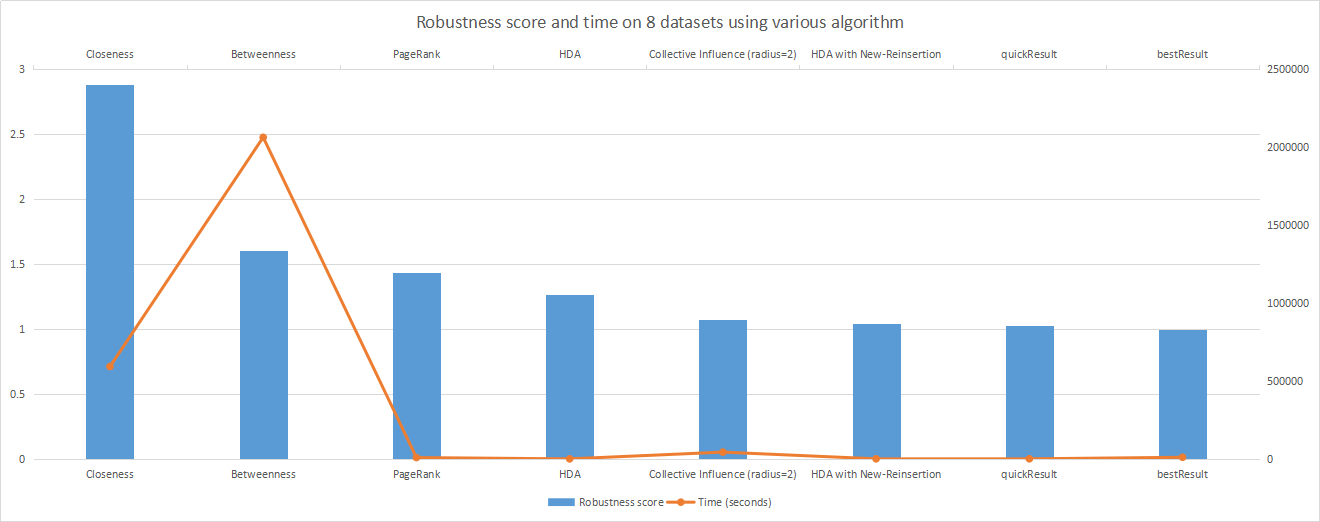
\includegraphics[width = 14cm]{3.png}
	\caption{Robustness score and time on 8 datasets using various algorithm}
	\label{fig:figure3}
	\end{figure}	
	
	
	The new proposed Generic reinsertion framework can achieve different goals according to the various kernels. In fact, for this issue in the Competition, kernel \textit{New-Reinsertion} , \textit{Trad-Reinsertion} and \textit{multiply-Reinsertion} are all implemented to recover the network as late as possible. In the future, more kernels need to be investigated to see whether the framework can be applied on the other issues. For example, we can develop the new kernel in order to recover the attacked and collapsed network as soon as possible, such the case that terrorist attacks on transportation or electric power supply. 
	


	
	%----------------------------------------------------------------------------------------
	%	BIBLIOGRAPHY
	%----------------------------------------------------------------------------------------
	
	\bibliographystyle{abbrv}
	
	\bibliography{sample}
	
	%----------------------------------------------------------------------------------------
	
	
\end{document}